\documentclass{ximera}
\newcommand{\RR}{\mathbb R}
\renewcommand{\d}{\,d}
\newcommand{\dd}[2][]{\frac{d #1}{d #2}}
\renewcommand{\l}{\ell}
\newcommand{\ddx}{\frac{d}{dx}}
\newcommand{\dfn}{\textbf}
\newcommand{\eval}[1]{\bigg[ #1 \bigg]}

%\author{Tom Dinitz and Nela Lakos}
\license{Creative Commons 3.0 By-NC}
\title{Formula Sheet}

\begin{document}
\begin{abstract}
\end{abstract}
\maketitle
\begin{image}
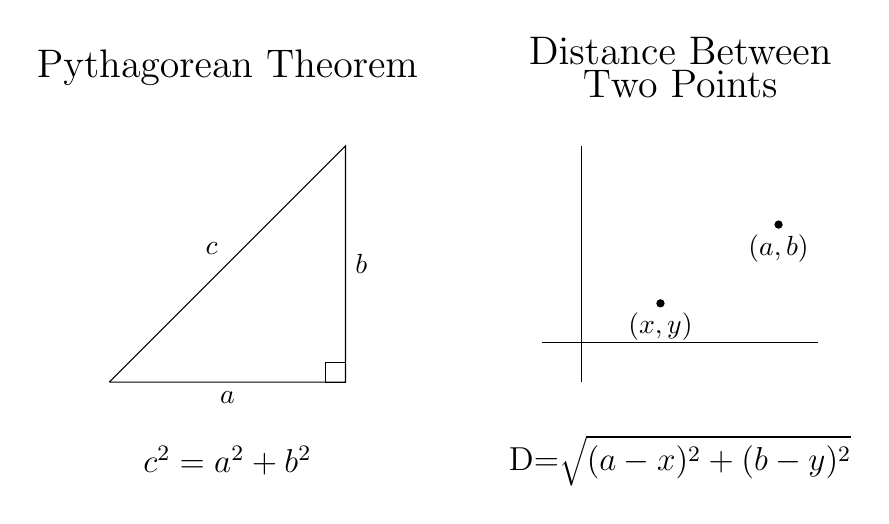
\begin{tikzpicture}
%Pyth Thm
  \node at (1.5,4) [align=center] {\Large Pythagorean Theorem}; 
\draw (0,0) -- node[below,pos=.5]{$a$}(3,0) -- node[right,pos=.5]{$b$}(3,3)-- node[above left,pos=.5]{$c$}(0,0);
\draw (3,0) rectangle (2.75,.25);
\node at (1.5,-1) [align=center] {\large $c^2=a^2+b^2$};

\node at (7.25,4) [align=center] {\Large Distance Between\\ \Large Two Points}; 
\draw (5.5,.5) -- (9,.5);
\draw (6,0) -- (6,3);
 \fill[fill=black] (7,1) circle (1.5pt) node[below]{$(x,y)$};
 \fill[fill=black] (8.5,2) circle (1.5pt) node[below]{$(a,b)$};
\node at (7.25,-1) [align=center] {\large D=$\sqrt{(a-x)^2+(b-y)^2}$};
\end{tikzpicture}
\end{image}
PERIMETERS AND AREAS
\begin{image}
  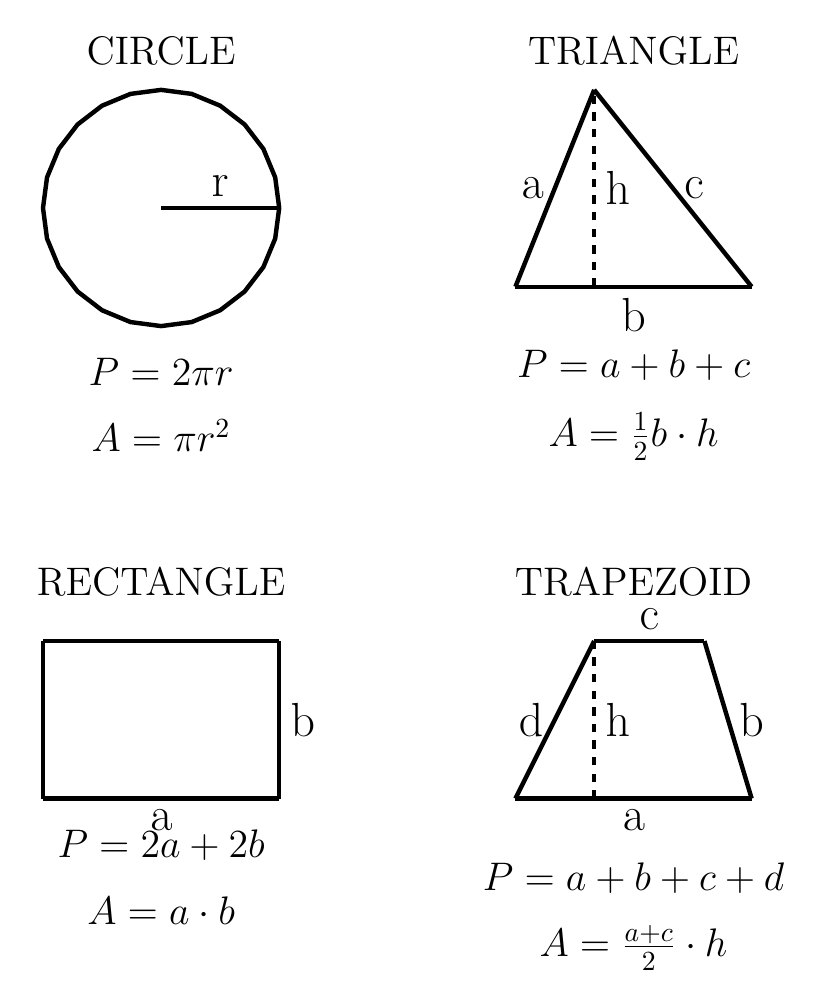
\begin{tikzpicture}
   %CIRCLE
   \node at (1.5,11.5) [align=center] {\Large CIRCLE};
    \draw [ultra thick,domain=0:360] plot ({1.5*cos(\x)+1.5}, {1.5*sin(\x)+9.5});
    \draw [ultra thick](1.5,9.5) -- (3,9.5) node[pos=0.5, above]{\LARGE r};
    \node at (1.5,7) [align=center] {\Large $P=2\pi r$\\\\ \Large $A=\pi r^2$};

    %\draw [penColor,ultra thick,domain=270:360] plot ({2*cos(\x)+8}, {2*sin(\x)+11});
    %\draw [penColor,ultra thick,domain=0:90] plot ({2*cos(\x)+2}, {2*sin(\x)+3});
    %\draw [penColor,ultra thick,domain=180:90] plot ({2*cos(\x)+10}, {2*sin(\x)+3});
 
    %TRIANGLE    
	\node at (7.5,11.5) [align=center] {\Large TRIANGLE};
	\draw [ultra thick] (6,8.5) -- (9,8.5) node[pos=0.5, below]{\LARGE b};
 	\draw [ultra thick] (6,8.5) -- (7,11) node[pos=0.5, left]{\LARGE a};
 	\draw [ultra thick]  (7,11) -- (9,8.5) node[pos=0.5, right]{\LARGE c};
	\draw [ultra thick, dashed]  (7,8.5) -- (7,11) node[pos=0.5, right]{\LARGE h};
 	\node at (7.5,7) [align=center] {\Large $P=a+b+c$\\\\ \Large $A=\frac{1}{2}b
	\cdot h$};
	

    %RECTANGLE
        \node at (1.5,4.75) [align=center] {\Large RECTANGLE};
	\draw [ultra thick] (0,2) -- (3,2) node[pos=0.5, below]{\LARGE a};
 	\draw [ultra thick] (3,2) -- (3,4) node[pos=0.5, right]{\LARGE b};
 	\draw[ultra thick]  (3,4) -- (0,4);
	\draw [ultra thick] (0,4) -- (0,2);
	
	\node at (1.5,1) [align=center] {\Large $P=2a+2b$\\ \\\Large $A=a\cdot b$};
	
	%TRAPEZOID
	\node at (7.5,4.75) [align=center] {\Large TRAPEZOID};
	\draw [ultra thick] (6,2) -- (9,2) node[pos=0.5, below]{\LARGE a};
 	\draw [ultra thick] (9,2) -- (8.4,4) node[pos=0.5, right]{\LARGE b};
 	\draw[ultra thick]  (8.4,4) -- (7,4)node[pos=0.5, above]{\LARGE c};
	\draw [ultra thick] (7,4) -- (6,2)node[pos=0.5, left]{\LARGE d};
	\draw[dashed,ultra thick]  (7,2) -- (7,4) node[pos=0.5,right] {\LARGE h};
	\node at (7.5,0.5) [align=center] {\Large $P=a+b+c+d$\\ \\\Large $A=\frac{a+c}{2}\cdot h$};
	
 \end{tikzpicture}
 \end{image}
 \pagebreak
 VOLUMES AND SURFACE AREAS
  \begin{image}
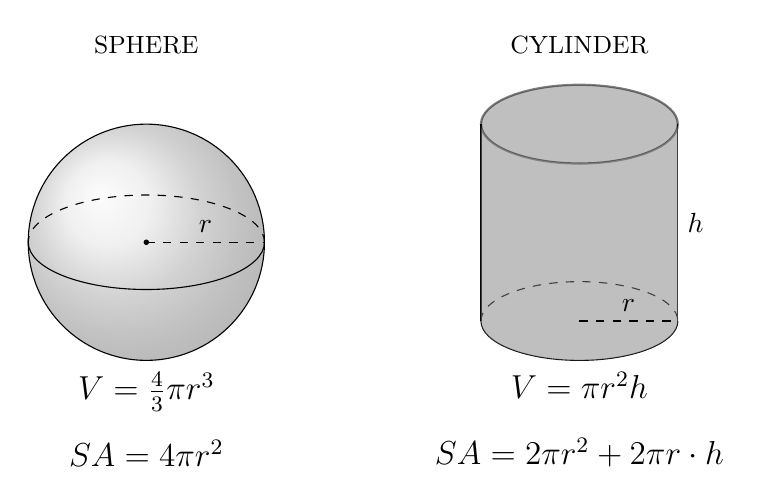
\begin{tikzpicture}
%SPHERE
  \node at (1.5,2.5) [align=center] { \small{SPHERE}};
  \shade[ball color = gray!40, opacity = 0.4] (1.5,0) circle (1.5);
  %\node at (0,0) [align=center]{a};
  \draw (1.5,0) circle (1.5cm);
  \draw (0,0) arc (180:360:1.5 and 0.6);
  \draw[dashed] (3,0) arc (0:180:1.5 and 0.6);
  \fill[fill=black] (1.5,0) circle (1pt);
  \draw[dashed] (1.5,0 ) -- node[above]{$r$} (3,0);
  
  \node at (1.5,-2.25) [align=center] {\large $V=\frac{4}{3}\pi r^3$\\ \\\large $SA=4\pi r^2$};
  
  %CYLINDER
  \node at (7,2.5) [align=center] { \small{CYLINDER}};
\draw [fill=gray,opacity=.5,thick](7,1.5) ellipse (1.25 and 0.5);
\draw (5.75,1.5) -- (5.75,-1);
\draw (5.75,-1) arc (180:360:1.25 and 0.5);
\draw [dashed] (5.75,-1) arc (180:360:1.25 and -0.5);
\draw (8.25,1.5) -- (8.25,-1) node[right,pos=.5]{$h$};  
\fill [gray,opacity=0.5] (5.75,1.5) -- (5.75,-1) arc (180:360:1.25 and 0.5) -- (8.25,1.5) arc (0:180:1.25 and -0.5);
\draw[dashed](5.75+1.25,-1) -- (8.25,-1) node[above,pos=.5] {$r$};
\node at (7,-2.25) [align=center] {\large $V=\pi r^2h$\\ \\\large $SA=2\pi r^2+2\pi r\cdot h$};
\end{tikzpicture}
\end{image}

\begin{image}
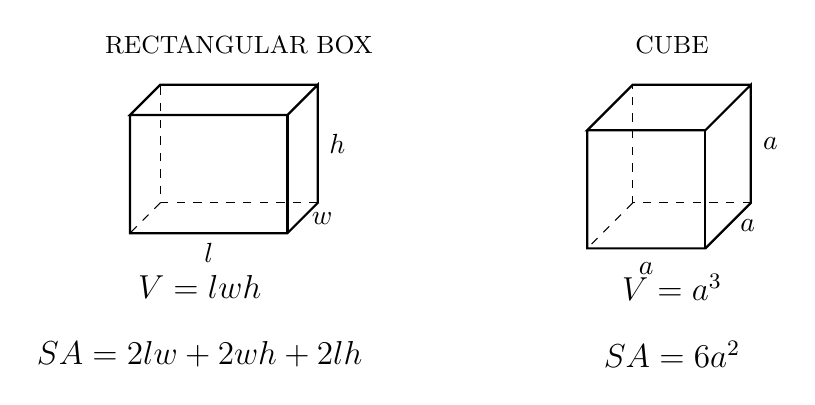
\begin{tikzpicture}

%BOX
  \node at (2.5,.5) [align=center] { \small{RECTANGULAR BOX}};
\pgfmathsetmacro{\xr}{3.5}
\pgfmathsetmacro{\xl}{1.5}
\pgfmathsetmacro{\yt}{0}
\pgfmathsetmacro{\yb}{-1.5}
\pgfmathsetmacro{\zi}{0}
\pgfmathsetmacro{\zo}{1}
  \draw[thick](\xr,\yt,0)--(\xl,\yt,\zi)--(\xl,\yt,\zo)--(\xr,\yt,\zo)--(\xr,\yt,\zi)--(\xr,\yb,\zi)--(\xr,\yb,\zo)--(\xl,\yb,\zo)--(\xl,\yt,\zo);
  \draw[thick](\xr,\yt,\zo)--(\xr,\yb,\zo);
  \draw[dashed](\xr,\yb,\zi)--(\xl,\yb,\zi)--(\xl,\yt,\zi);
  \draw[dashed](\xl,\yb,\zi)--(\xl,\yb,\zo);
  \draw(\xr+.25,\yt*.5+\yb*.5,\zi) node{$h$};
  \draw(\xr+.25,\yb,\zi*.5+\zo*.5) node{$w$};
  \draw(\xl*.5+\xr*.5,\yb-.25,\zo) node{$l$};
\node at (2,-3) [align=center] {\large $V=lwh$\\ \\\large $SA=2lw+2wh+2lh$};  
  
  %CUBE
    \node at (8,.5) [align=center] { \small{CUBE}};
  \pgfmathsetmacro{\cxr}{9}
\pgfmathsetmacro{\cxl}{7.5}
\pgfmathsetmacro{\cyt}{0}
\pgfmathsetmacro{\cyb}{-1.5}
\pgfmathsetmacro{\czi}{0}
\pgfmathsetmacro{\czo}{1.5}
  \draw[thick](\cxr,\cyt,0)--(\cxl,\cyt,\czi)--(\cxl,\cyt,\czo)--(\cxr,\cyt,\czo)--(\cxr,\cyt,\czi)--(\cxr,\cyb,\czi)--(\cxr,\cyb,\czo)--(\cxl,\cyb,\czo)--(\cxl,\cyt,\czo);
  \draw[thick](\cxr,\cyt,\czo)--(\cxr,\cyb,\czo);
  \draw[dashed](\cxr,\cyb,\czi)--(\cxl,\cyb,\czi)--(\cxl,\cyt,\czi);
  \draw[dashed](\cxl,\cyb,\czi)--(\cxl,\cyb,\czo);
  \draw(\cxr+.25,\cyt*.5+\cyb*.5,\czi) node{$a$};
  \draw(\cxr+.25,\cyb,\czi*.5+\czo*.5) node{$a$};
  \draw(\cxl*.5+\cxr*.5,\cyb-.25,\czo) node{$a$};
\node at (8,-3) [align=center] {\large $V=a^3$\\\\ \large $SA=6a^2$};  
 \end{tikzpicture}
  \end{image}

\begin{image}
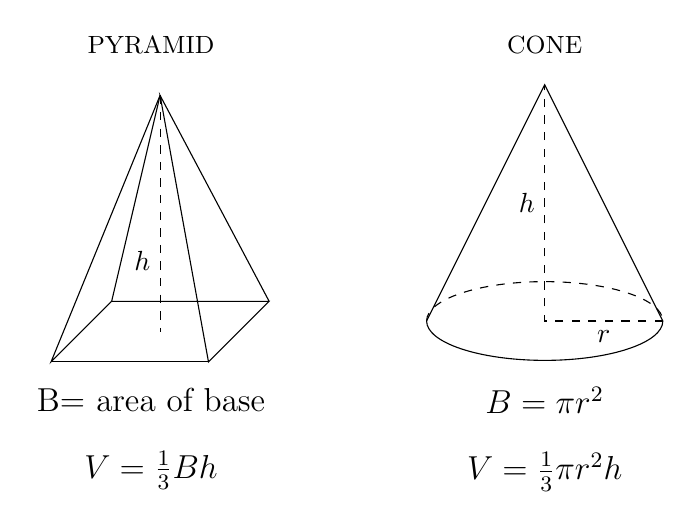
\begin{tikzpicture}
%PYRAMID
  \node at (1.5,3.25) [align=center] { \small{PYRAMID}};
    \draw (2,3,1) -- (1,0,0) -- (3,0,0) -- (3,0,2) -- (2,3,1) 
      -- (3,0,0);
    \draw (2,3,1) -- (1,0,2) 
      -- (1,0,0);
    \draw(1,0,2) -- (3,0,2);
    \draw (5.6,-.2,2);
    \draw[dashed](2,3,1) -- node[left,pos=.7] {$h$} (2,0,1);

 \node at (1.5,-1.75) [align=center] {\large B= area of base\\\\ \large $V=\frac{1}{3}Bh$}; 
 
%CONE 
  \node at (6.5,3.25) [align=center] { \small{CONE}}; 
\pgfmathsetmacro{\ys}{-.25}
\draw 
  (5,0+\ys) arc (180:360:1.5 and .5) -- (6.5,3+\ys) -- cycle;
\draw[dashed]
  (5,0+\ys) arc (180:0:1.5 and .5);
\draw[dashed]
  (8,0+\ys) -- node[below] {$r$} (6.5,0+\ys) -- node[left] {$h$} (6.5,3+\ys) ;
  \node at (6.5,-1.5+\ys) [align=center] {\large $B= \pi r^2$\\ \\\large $V=\frac{1}{3}\pi r^2h$}; 
\end{tikzpicture}
\end{image}
\pagebreak
\begin{center}
\Large {Trig Functions of Some Special Angles}
\end{center}
\[
{\LARGE{\begin{tabular}{|| c || c || c || c || c || c ||}\hline\hline
\color{blue}{ANGLE}& \color{blue}{0} & \color{blue}{$\pi / 6$} & \color{blue}{$\pi / 4$} & \color{blue}{$\pi / 3$} & \color{blue}{$\pi / 2$} \\ \hline\hline
 $\sin(\theta)$ & 0 & $1 / 2$ & $1/\sqrt{2}$& $\sqrt{3}/2$ &1\\

\hline
$\cos(\theta)$ & 1 & $\sqrt{3}/2$ & $1/\sqrt{2}$& $1/2$ &0\\

\hline 
$\tan(\theta)$ & 0 & $1/\sqrt{3}$ & 1& $\sqrt{3}$ & DNE \\

\hline 
$\cot(\theta)$ & DNE & $\sqrt{3}$ & 1& $1/\sqrt{3}$ & 0 \\\hline
$\sec(\theta)$ & 1 & $2/\sqrt{3}$ & $\sqrt{2}$& $2$ &DNE \\ \hline
$\csc(\theta)$ & DNE & $2$ & $\sqrt{2}$& $2/\sqrt{3}$ &$1$\\\hline 
\end{tabular}}}
\]
\pagebreak
\begin{center}
{\Large Famous Trig Identities}
\end{center}


$\tan(\theta)=\frac{\sin(\theta)}{\cos(\theta)}$, \text{          }$\cot(\theta)=\frac{\cos(\theta)}{\sin(\theta)}$\\

$\sec(\theta)=\frac{1}{\cos(\theta)}$, \text{           }$\csc(\theta)=\frac{1}{\sin(\theta)}$\\

$\cos^2(\theta)+\sin^2(\theta)=1$\\

$1+\tan^2(\theta)=\sec^2(\theta)$\\\\



$\sin(\alpha+\beta)=\sin(\alpha)\cos(\beta)+\cos(\alpha)\sin(\beta)$\\

$\sin(\alpha-\beta)=\sin(\alpha)\cos(\beta)-\cos(\alpha)\sin(\beta)$\\

$\cos(\alpha+\beta)=\cos(\alpha)\cos(\beta)-\sin(\alpha)\sin(\beta)$\\

$\cos(\alpha-\beta)=\cos(\alpha)\cos(\beta)+\sin(\alpha)\sin(\beta)$\\\\




$\tan(\alpha+\beta)=\frac{\tan(\alpha)+\tan(\beta)}{1-\tan(\alpha)\tan(\beta)}$\\\\\\
$\tan(\alpha-\beta)=\frac{\tan(\alpha)-\tan(\beta)}{1+\tan(\alpha)\tan(\beta)}$\\\\\\



$\sin(2\theta)=2\sin(\theta)\cos(\theta)$\\

$\cos(2\theta)=\cos^2(\theta)-\sin^2(\theta) = 2\cos^2(\theta)-1 = 1-2\sin^2(\theta)$\\\\

$\sin\left(\frac{\theta}{2}\right)=\pm\sqrt{\frac{1-\cos(\theta)}{2}}$\\

$\cos\left(\frac{\theta}{2}\right)=\pm\sqrt{\frac{1+\cos(\theta)}{2}}$\\

$\tan\left(\frac{\theta}{2}\right)=\frac{\sin(\theta)}{1+\cos(\theta)}=\frac{1-\cos(\theta)}{\sin(\theta)}$

\end{document}